\chapter{State consensus through anti-entropy}
\label{chap:mechanism}
% A specific implementation of the extension of TrustChain

% A policy that makes dissemination and verificaiton strategy-proof
In the first chapters of this thesis we introduced the incentive problem of information dissemination 
in distributed reputation systems. In the previous chapter we introduced an extension of the TrustChain
architecture that allows for agents in the network to obtain and verify each other's internal 
information state. But in order to achieve the goal of strategy-proof dissemination of information
a tangible mechanism is required that applies the advanced tools that the new architecture provides.
In this chapter we analyze one such mechanism which is based on the anti-entropy concept. We first
describe the mechanism conceptually, then discuss the implementation details and finally elaborate
on some intrinsic properties the mechanism could introduce in actual applications. In the next
chapter an implementation will be analyzed experimentally with small agent sets in order to prove
that properties from the theoretical analysis can be observed in practice.

\section{Conceptual description}
% The exact protocol: before each transaction we exchange all data and verify each other's chain

% What this allows us to do is: we can agree on a ranking that includes all of both agents data. 

% We give the receiver a chance to proof that he is worth

% We make sure that an agent has to obtain all data before making a transaction. 
Section~\ref{sec:strategy_proof_sharing} explained that the architecture itself does not solve the 
incentive problem. It rather provides the evidence on which an incentive mechanism can be built. 
Many different mechanism are possible, depending on the specific needs of the application context. 
This offers a lot of flexibility for system designers which is different from existing architectures
which a very static in their protocol and have pre-defined security and scalability properties.

\subsection{Design choice: security vs scalability}
Security, decentralization and scalability are three properties that are traded against each other 
in the design of a decentralized system. It can be argued that TrustChain was designed with scalability
as the highest priority while Bitcoin was designed with security as highest priority property. We
argue that the extension that allows for internal agent state transparency allows for flexibility in
the design choice of security and scalability. In this section we propose a mechanism that trades 
some of the scalaiblity of TrustChain for stronger security in order to show that a secure mechanism
is possible on top of the TrustChain architecture. 

\subsection{Concept: anti-entropy}
The mechanism is based on the concept of anti-entropy, which was described in \cite{demers1987epidemic}
for the purpose of maintaining mutual consistency between multiple replicas of a database. Updates
to the database can arrive at any single site and need to be forwarded to all other replicas. Demers
et. al. study three different mechanisms to disseminate the updates to other sites: direct mail, 
anti-entropy and rumor mongering.

In the direct mail mechanism, a database forwards the update to all other database immediately, which
seems like the most straight forward approach but is restricted by the fact that each database does
not know about all other databases. 

Anti-entropy is a process in which each database periodically chooses a partner database and both 
exchange all database contents in order to resolve any differences between the two. The process was
found to be reliable but slower than direct mail. 

The final mechanism is called Rumor Mongering. Sites consider updates ``hot rumors'' after receiving
them for the first time. While the site considers the rumor ``hot'', it choses periodically another
site and informs it about the rumor. When the site has encountered a certain amount of sites which
were already aware of the ``hot rumor'', that update is retained but site stops with actively
propagating the update. 

For the purpose of this work, we will focus on the concept of anti-entropy. Direct mail is not a
viable option because for large social networks the embedded social networks are a very small 
subset and the rest of the agents in the network would not be informed of updates. Rumor mongering 
effects are best observed in larger networks however this work is concerned with conceptual analysis
and the experimental analysis in the next section concerns small networks. Also there are more 
algorithms than these three but anti-entropy fits the architecture of TrustChain very well and is 
a good starting point for analyasis of dissemination mechanisms. The analysis of other mechanisms
will be subject of future work.

\subsection{Replicated databases vs TrustChain}
The context of the work of Demers et. al. is similar to the context that this work is concerned with
in many regards. Replicated databases are a distributed system as all instances of the database are
independent, equal entities, just like the agents in the TrustChain network. Each agent has an 
internal state which is equal to the set of transactions that agent is aware of which is equal to
the state of the database which is equal to the entries that database is aware of. Our goal is to 
propagate information on new transactions just like the goal of Demers et. al. was to propagate 
updates to the databases. 

In the context of reputation systems anti-entropy allows for two agents to align on their knowledge
of the social network, that is to obtain the same embedded social network and agree on the reputation
of all agents in that network.
Two agents, $a_i$ and $a_j$ have two different internal states, represented by the sets of encounters
$E_i$ and $E_j$. There can be some overlap between the two sets, but that is not guaranteed. Agent 
$a_i$ chooses to synchronize states with agent $a_j$. Both agents send their own set of known 
encounters and merge them. This results in a new set $E_{i,j} = E_i \bigcup E_j$. In the context 
of TrustChain this translates to the exchange of transaction blocks, such that after the exchange 
both agents have the exact same set of transaction blocks. As the reputation of peers is calculated
from the set of transactions both agents agree on a single reputation vector. If the two agents also
use the same function for trust calculation both can even agree on a single trust vecotr. The two 
agents have reached consensus on trust and reputation. 

The exchange of information will be recorded in the form of exchange blocks on the chain of both 
participating agents as explained in the previous chapter, section~\ref{sec:implementation_state_transparency}.

The consensus is only reached at one point in time and is not maintained. Once any of the two agents
conducts another anti-entropy exchange or a transaction, the other agent is not required to be 
informed or to observe the interaction. That is after the exchange both internal states can diverge
until the same two agents happen to perform another state synchronization. 

In the work of Demers et. al. database instances chose partners for anti-entropy exchanges at random
which is a valid strategy as each peers updates seem equally important. In contrast, reputation 
systems should value the information about possible future interaction partners as more important.
Therefore, our proposed mechanism requires agents to at least perform an anti-entropy exchange with
those agents that they will have an interaction next. That way, both parties of a transaction are 
required to obtain and verify each others information in order to make sure that the transaction 
will be done on top of a valid state. If any party does not agree with the state of the opposite 
party, the transaction will not take place. If any party performs a transaction eventhough the 
information clearly shows misconduct on the part of the partner, they will also be held responsible 
for not performing their validation responsibility. Without the requirement of validating transaction
partners, agents can purposefully exchange data with honest agents but perform interactions with 
dishonest agents and later claim to have had no knowledge of the dishonesty of the partners. 

\section{Implementation of anti-entropy exchanges}
In the previous section we described the anti-entropy method for information exchanges between 
agents. This section elaborates on the implementation details of the mechanism in the TrustChain 
architecture. We start with an application agnostic example of the exchange of information and the 
transaction process.. In the next section we expand on the considerations for application specific 
implementations.

We consider an agent $a_i$, who is about to conduct another interaction. What the interaction is 
about and how the partner is chosen are specific to the application context. For this example we 
assume that $a_i$ can randomly choose an agent from the network. Once $a_i$ has chosen a partner $a_j$,
$a_i$ starts the communication and is therefore the \textit{initiator} while $a_j$ is the \textit{responder}. 

The initiator starts the interaction by sending the chain and exchange history to the responder. The
chain{\color{red} Is this explained somewhere} includes the blocks that describe the transaction and 
exchange history {\color{red} Is this explained somewhere} of the initiator while the exchange 
history includes the index of blocks exchanged for each exchange block. On reception, the responder 
can verify the chain using the algorithm \ref{alg:verify_chain}. The algorithm first checks,
wether the chain is a complete sequence without missing blocks in between. If the check is positive,
the number of exchange and transaction blocks is compared, as well as the public keys of partners
such that each transaction can be paired with a succesful exchange previous to the transaction.

\begin{algorithm}
\caption{Chain }\label{alg:verify_chain}
\begin{algorithmic}[1]
\Procedure{verifyChain}{}
\EndProcedure
\end{algorithmic}
\end{algorithm}

Once that check also succeeds, the responder is able to build a block index that indexes the internal
state of an agent. The block index is a summary of the contents of the internal state and shows
which transactions of which agents are knwon to the agent. This is an optimization that allows agent
to request only specific blocks instead of the complete database of another agent. This is a lot 
faster if agents that already share a lot of data. Agent $a_j$ compares the calculated block index
with his own index and request the difference in blocks, so those that $a_i$ has but $a_j$ does not 
have from $a_i$.

The initiator receives the request and replies with the blocks that $a_j$ requires to perform the 
complete internal state validation. Should the responder, for whatever reason, wrongly require more
blocks, so also blocks that are not in $a_i$'s posession, the interaction will be canceled. 

The responder receives the missing blocks. At this point $a_j$ should be in the posession of all
of $a_i$'s blocks plus some blocks that $a_j$ has over $a_i$. Agent $a_j$ is then able to perform
the complete internal state verification according to algorithm~\ref{alg:verify_state}. A state is
valid if:

\begin{algorithm}
    \caption{Chain }\label{alg:verify_state}
    \begin{algorithmic}[1]
    \Procedure{verifyChain}{}
    \EndProcedure
    \end{algorithmic}
\end{algorithm}

\begin{itemize}
    \item the chain is valid as per algorithm~\ref{alg:verify_chain}
    \item the hashes of the blocks according the the exchange indexes match the hashes recorded on
    the chain's exchange blocks
    \item Any recorded misbehavior of other agents is reflected by those agents' public keys in the 
    ignore and block list
\end{itemize}

If the internal state of $a_i$ is determined to be valid by $a_j$, the responder shows approval by 
sending the own chain, exchange history and blocks (which can be calculted by taking the opposite
difference from before) to agent $a_i$. 

Once the initiator receives that data from the responder, the second validtion of chain and state, 
this time agent $a_j$ as subject, can be conducted. If also this checks out, the valdiation phase is 
completed and the initiator can publish an exchange block proposal, which includes the hashes of the
exchanged blocks. The responder receives that proposal and the hashes contained in the proposal block
match the hashes that $a_j$ calculates for the excahnged data, the block is signed and returned.

This concludes the anti-entropy exchange, after this the two agents perform a normal interaction.

\section{Example}

In order to make the mechanism clearer, an example is provided in this section. We look at two
agents, Alice and Bob. Alice wants to interact with Bob and starts the interaction. We assume that
both agents are new to the network and only have their genesis blocks on the chain. In order to
start the interaction, Alice sends her chain (only the genesis block) and an empty set of exchanges
to Bob. Obviously the genesis block is accepted and Bob shows his approval by sending his own
genesis block and an empty set of exchanges. Also Alice accepts the data and creates an exchange 
block proposal. Figure \ref{fig:exchange_example} shows the chains of Alice and Bob after the 
complete interactions. The block proposal is Alice's block 2. When Bob receives the block, he checks
that the exchange hashes in the proposed exchange block match the hashes of the two genesis blocks 
from Alice and himself. If he agrees, he documents the acquisition of the exchange block in a
single-signed exchange block (Bob's block 2) and creates the agreement block (Bob's block 3) to the exchange block proposal. He 
sends back the exchange block agreement to Alice, who herself creates a single-signed exchange block
(Alice's block 3) for the acquisition of the exchange agreement block. At this point Alice is ready for the actual 
transaction. How the transaction happens exactly is not of importance for this example. After the transaction was successfully conducted it also needs to be documented. Again,
the same process as with the exchange is followed. Alice creates a transaction block proposal (Alice's block 4), Bob
creates the acquisition block and the agreement block (Bob's block 4 and 5). Finally, Alice creates the acquisition block of the agreement block of the transaction.

\begin{figure}
    \centering
    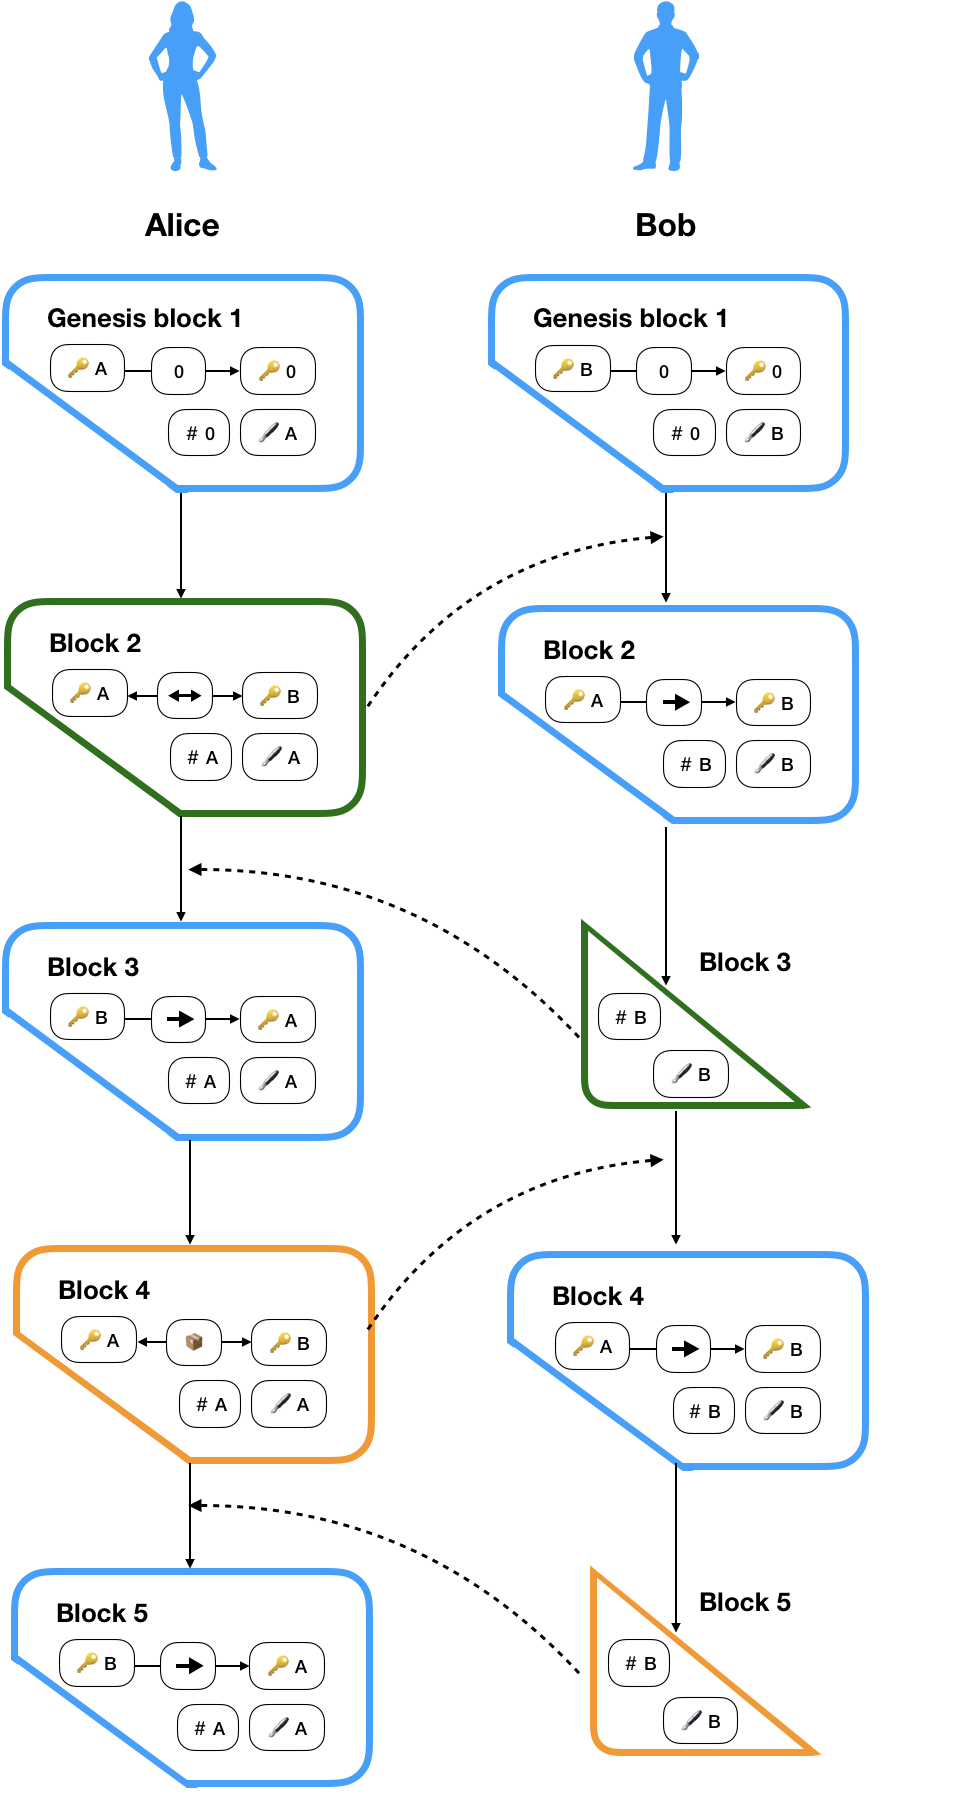
\includegraphics[height=0.9\textheight]{images/exchange_example}
    \caption{Example of one interaction between two agents}
    \label{fig:exchange_example}
\end{figure}

This example sheds light on the block creation process but is too simple to properly explain the 
exchange and verification process. We extend the example with another agent, Charles, whom Bob would
like to interact with after the previous interactions. Again, Charles is assumed to be new to the 
network so the genesis block is the only block on his chain. Bob starts the interactions by sending
his chain and exchanges. Now Charlie performs some checks: 

\begin{itemize}
    \item \textit{Is the chain complete?} - the chain is a full sequence (1 through 5) and Charlie 
    is not aware of any later blocks than 5, so the chain seems valid
    \item \textit{Are the exchanges correct?} - there are three exchange blocks on the chain, one
    receiving the exchange block proposal, one for the actual exchange of the genesis block of A and
    one for the transaction block proposal. Charlie recalculates the hashes stored in the exchange 
    blocks from the blocks sent by Bob. If all the hashes are equal, the exchanges are accepted.
\end{itemize}

Once Charlie accepts all the checks, he sends his own chain and exchanges which are checked by Bob
and the interaction continues as previously described. Table \ref{tab:blocks_example} shows the
blocks that each agent has after the first and second round. After the second round, Charles has 
all the blocks from Bob that he had after the first round.

\begin{table}[h!]
    \centering
    \caption{The block databases of each agent for the example}
    \label{tab:blocks_example}
    \begin{tabular}{p{4cm}|p{3cm}|p{4cm}|p{3cm}}
        \toprule
        Database & Alice & Bob & Charles \\
        \midrule
        Before first round & A: $[1]$ & B: $[1]$ & C: $[1]$ \\ \hline 
        After first round & A: $[1, 2, 3, 4, 5]$ \newline B: $[1, 3, 5]$ & A: $[1, 2, 4]$ \newline B: $[1, 2, 3, 4, 5]$ & C: $[1]$ \\ \hline
        After second round &  A: $[1, 2, 3, 4, 5]$ \newline B: $[1, 3, 5]$ & A: $[1, 2, 4]$ \newline B: $[1, 2, 3, 4, 5, 6, 7, 8, 9]$ \newline C: $[1, 3, 5]$ & A: $[1, 2, 4]$ \newline B: $[1, 2, 3, 4, 5, 6, 8]$ \newline C: [1, 2, 3, 4, 5] \\
        \bottomrule
    \end{tabular}
\end{table}

In order to make even clearer how the implementation works internally, Table \ref{tab:exchange_blocks}
shows which mappings of exchange blocks to exchanged blocks exist.

\begin{table}[h!]
    \centering
    \caption{All exchange blocks with their corresponding exchanged blocks}
    \label{tab:exchange_blocks}
    \begin{tabular}{l| p{5cm}}
        \toprule
        Block & Exchanged blocks \\
        \midrule
        Alice Block 2    & B: $[1]$ \\
        Alice Block 3    & B: $[3]$ \\
        Alice Block 5    & B: $[5]$ \\
        Bob Block 2      & A: $[2]$ \\
        Bob Block 3      & A: $[1]$ \\
        Bob Block 4      & A: $[4]$ \\
        Bob Block 6      & C: $[1]$ \\
        Bob Block 7      & C: $[3]$ \\
        Bob Block 9      & C: $[5]$ \\
        Charles Block 2  & B: $[6]$ \\
        Charles Block 3  & A: $[1, 2, 4]$, B: $[1, 2, 3, 4, 5]$ \\
        Charles Block 4  & B: $[8]$ \\
        \bottomrule
    \end{tabular}
\end{table}

\section{Consideration of application specific features}
choosing partners -- we now chose partners randomly but probably for many applications there are 
better strategies
application specific rules -- we could perform additional verification for application context, for
example no downloading after a certain negative balance boundary

\section{Advanced implications of anti-entropy}
locality -- when you need to exchange all information and storage has value, it is cheaper to 
interact with agents that have a largely similar information set
sybil attack -- when we can apply application specific rules and we require agents to perform checks
of all agents they interact with, we can introduce a rule that says agents cannot upload to agents
that are completely new to the network (they first have to prove themselves). This way an agent 
cannot create fake agents that all download from one agent and thus increase that agents balance 
without actual downloading happening
